\chapter[Librairie d'arbres]{Implémentation d'une librairie sur les arbres%
\chaptermark{Librairie d'arbres}}
Étant donné le retard pris par nos deux binôme dans la réalisation du projet, nous avons préféré effectuer une analyse sur une hiérarchie permettant de représenter les différentes implémentations d'arborescences plutôt que d'essayer de produire du code qui ne serait certainement pas terminé au terme de ce projet.

Dans un premier temps nous proposerons donc un modèle de hiérarchie sur les arborescences qui pourrait permettre, par la suite, une éventuelle implémentation d'une librairie. Puis nous discuterons sur les moyens pouvant être mis en oeuvre pour automatiser le choix des structures.

\section{Une possible hiérarchie sur les arbres%\sectionmark{Hiérarchie}%
}
\sectionmark{Hiérarchie}
\paragraph{Introduction} Dans cette partie, nous allons détailler une hiérarchie d'arborescence qui nous paraît plausible. Pour vous permettre de visualiser cette dernière plus aisément reportez vous à la figure \ref{fig:hierarchie} 
\begin{landscape}
\begin{figure}[h]
	\centering
	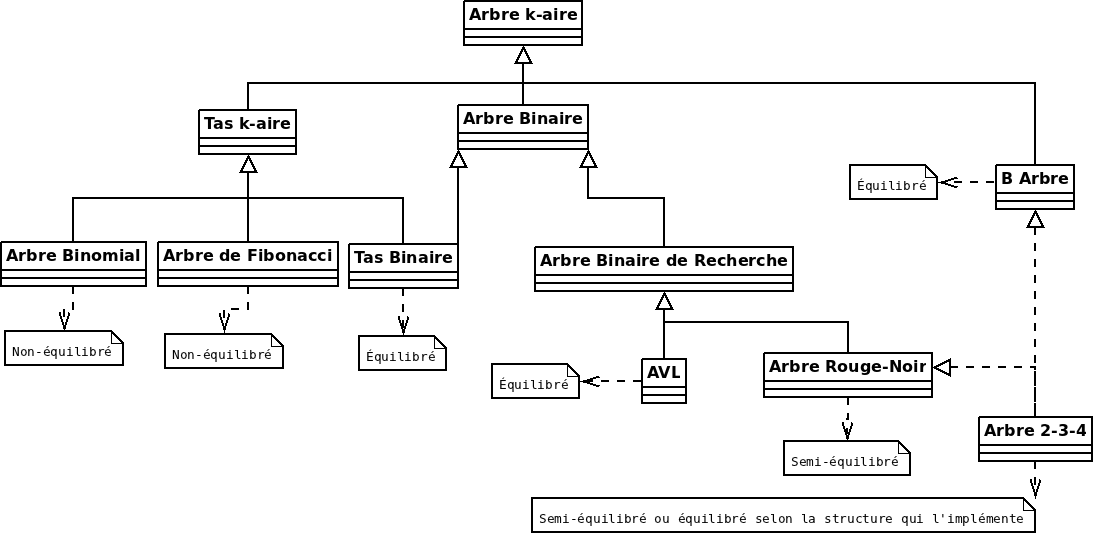
\includegraphics[scale=0.5]{Hierarchie_arbres}
	\caption{Une hiérarchie sur les arbres}
	\label{fig:hierarchie}
\end{figure}
\end{landscape}

\paragraph{Justification du modèle} 
\begin{description} 
\item[Arbre k-aire]Dans notre modèle, l'arbre k-aire est la classe/interface père de toutes les autres. Cette appellation n'est peut-être pas la plus pertinente puisqu'il s'agit en fait d'une structure arborescente ou chaque n\oe ud peut avoir $f$ fils et contenir $e$ éléments. Cette structure peut être une interface comme une classe concrète mais elle ne présente que peu d'intêret pour ce dernier cas puisqu'elle n'offre aucun avantage algorithme (complexité etc\dots )
\item[Arbre binaire] Il s'agit d'une spécification de l'arbre k-aire ou le nombre de n\oe uds ne peut contenir qu'un élément et ne posséder que deux fils (en excluant le cas des feuilles). Tout comme l'arbre k-aire, il sera sûrement implémenter comme une interface ou tout du moins comme une classe abstraite.
\item[Tas k-aire] La structure du tas spécifie l'arbre k-aire en forçant le nombre d'éléments dans chaque n\oe ud à un et en ajoutant la relation d'ordre entre la valeur du n\oe ud père et celle de ces fils. Là encore on peut imaginer qu'il s'agira d'une classe abstraite.
\item[B arbre] Le B arbre spécifie l'arbre k-aire en permettant de contenir dans un n\oe ud un nombre d'élément nécessairement compris entre $e$ et $\frac{e}{2}$. De plus le nombre de fils est dépendant du nombre $e'$ d'éléments présents à un moment donné dans le n\oe ud puisqu'il est au maximum de $e'+1$. Il s'agit d'ailleurs d'une classe concrète implémentée dans la première partie du sujet.
\end{description}

Toutes les structures suivantes peuvent être considéré comme étant à implémenter en tant que classes concrètes :
\begin{description} 
\item[Arbre binomial et de Fibonacci] Il s'agit de structures très proches du tas k-aire permettant, respectivement, l'implémentation d'un tas binomial et de Fibonacci.
\item[Tas binaire] Le tas binaire est une implémentation concrète possédant à la fois les propriétés des arbres binaires et celle des tas.
\item[Arbre binaire de recherche] Cette structure de données spécifie l'arbre binaire en imposant une organisation des valeurs dans l'arbre.
\item[AVL] L'AVL est une structure spécifiant l'arbre binaire de recherche en forçant celui-ci à être équilibré.
\item[Arbre rouge-noir] Spécification particulière de l'arbre binaire de recherche.
\item[Arbre 2-3-4] Il s'agit d'une structure de données pouvant être implémentée soit par un B arbre avec le nombre maximal d'élements dans un n\oe ud fixé à 4; soit par un arbre rouge-noir, ce dernier étant isomorphe à l'arbre 2-3-4.
\end{description}
